\documentclass[11pt]{article}

\usepackage[margin=1in]{geometry}
\usepackage{booktabs}
\usepackage{graphicx}
\usepackage{hyperref}

\hypersetup{
  colorlinks=true,
  linkcolor=blue,
  urlcolor=blue,
  citecolor=blue
}

\title{Weekly Report: PASTA Paper Revision and PTCL-Aware Translation Design}
\author{Daoxuan Xu}
\date{June 17, 2026}

\begin{document}
\maketitle

\section{Summary}

This week focused on revising the PASTA paper and reorganizing the major
technical contributions. The main change is to move away from presenting
coalescing as a standalone method. Instead, the paper will focus on two more
architectural mechanisms:

\begin{itemize}
  \item A locality-aware page placement policy that reduces pressure on the
        remote IOMMU/MMU translation path.
  \item A PTCL-aware TLB entry design that improves L2 TLB lookup and placement.
  \item A GPM-side translation prefetcher that predicts future PTCLs based on
        local and remote translation latency.
\end{itemize}

\section{Optimizing Page Placement Policy}

I first revisited page placement because the translation pressure traces show
that different workloads place very different pressure on the local GMMU page
walkers and the remote IOMMU/MMU path. From the 14 benchmark traces, I selected
three representative cases: ReLU, KMeans, and SPMV. ReLU is mostly served by
the local GMMU path, KMeans stresses both local and remote translation paths,
and SPMV is dominated by the remote IOMMU/MMU path. This imbalance suggests
that page placement is still an important optimization target.

The next design direction is a locality-aware page placement policy. The goal
is to place pages so that translations with strong locality are more likely to
be served by the local GMMU path. This should reduce remote translation
pressure, improve locality in the PTCL-aware TLB, and make the later PTCL entry
and prefetching mechanisms more effective.

\begin{figure}[t]
  \centering
  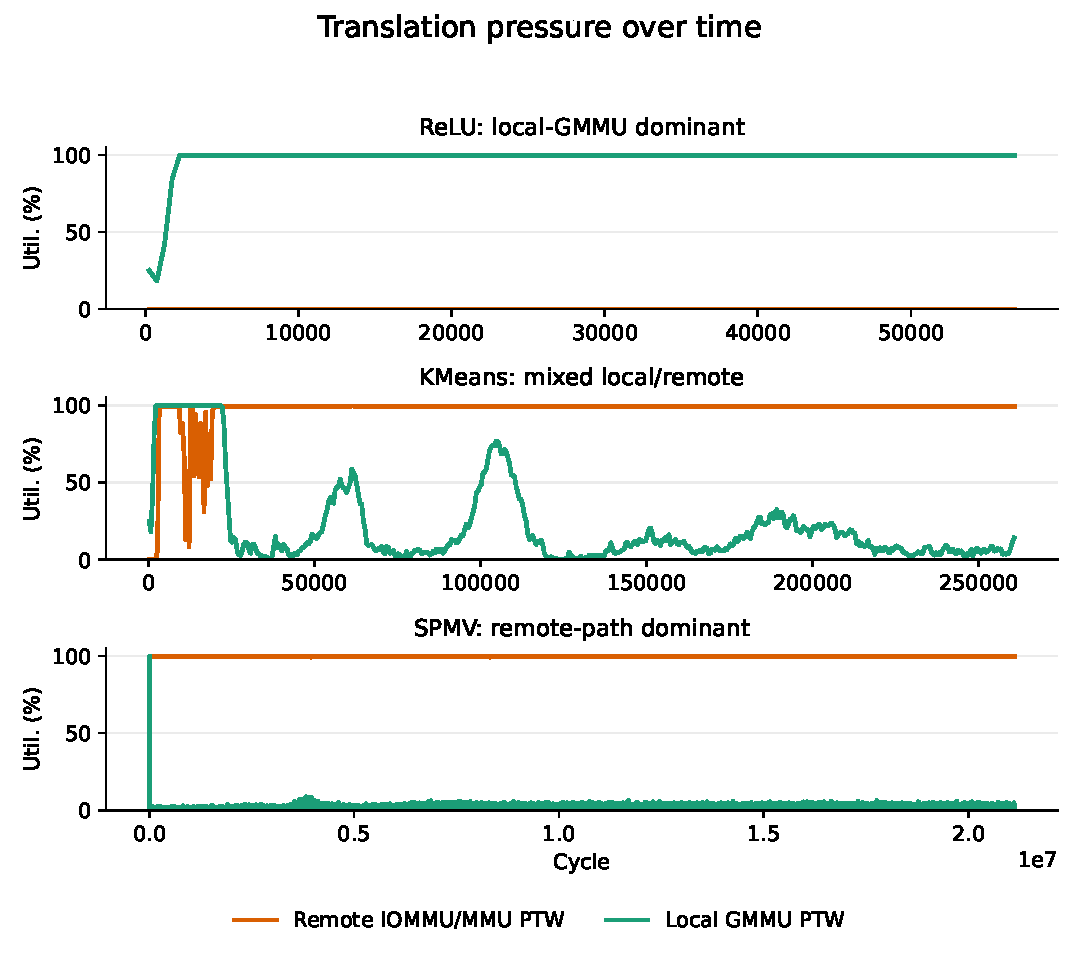
\includegraphics[width=\linewidth,height=0.58\textheight,keepaspectratio]{figures/translation_pressure_utilization.pdf}
  \caption{Translation pressure over time for three representative benchmarks
  selected from 14 traces. ReLU is local-GMMU dominant, KMeans is mixed, and
  SPMV is remote-path dominant. This motivates revisiting page placement with a
  locality-aware policy.}
  \label{fig:translation-pressure-page-placement}
\end{figure}

\section{PASTA Paper Revision}

The main paper-level change this week is the method organization. In the
previous version of PASTA, one major mechanism was Prefix-Aware Page-table
Walking. During the review process, this mechanism was challenged because its
novelty was not sufficiently clear relative to prior GPU address-translation
work. In particular, reviewer feedback pointed out the overlap with
Neighborhood-Aware Address Translation~\cite{shin2018neighborhood} and
LATPC~\cite{ha2025latpc}. Neighborhood-Aware Address Translation already
exploits page-table cache-line locality during IOMMU-side page-table walking,
while LATPC is another recent locality-aware GPU address-translation design.
Because these prior works make the novelty of Prefix-Aware Page-table Walking
harder to defend, I plan to remove it from the revised paper.

Instead, the revised paper will introduce PTCL TLB entry design as the new
second method. This method focuses on the L2 TLB entry access and placement
problem, which is different from prior work on page-table walking and request
locality. The goal is to make the contribution more clearly distinguishable:
PASTA redesigns how PTCL-granular translation state is represented and accessed
inside the GPU-side TLB.

The revised PASTA method structure is:

\begin{itemize}
  \item \textbf{Method 1: PTCL-aware translation request handling.}
        This includes PTCL-granular tracking, bitmap-based request state, and
        representative downstream requests. It provides the foundation for later
        optimizations.
  \item \textbf{Method 2: PTCL TLB entry design.}
        This replaces the previous coalescing-focused method. The goal is to
        make the L2 TLB entry organization aware of PTCL locality so that a
        PTCL request does not always need to behave like eight independent PTE
        lookups.
  \item \textbf{Method 3: GPM-side translation prefetcher.}
        This replaces the previous IOMMU-TLB-side prefetcher. The prefetcher is
        placed closer to the GPM/L2 TLB side so that it can react to GPU-side
        address translation requests earlier.
\end{itemize}

This reorganization makes the paper cleaner. Coalescing is still important, but
it becomes part of the PTCL request semantics rather than a standalone method.
The paper can then emphasize the two main optimizations that directly change
the TLB access path and the prediction path.

\section{PTCL TLB Entry Design}

The new second method is the PTCL TLB entry design. The motivation is that the
current PTCL request path can reduce downstream traffic, but the L2 TLB lookup
path may still behave like multiple independent PTE lookups. This creates a gap
between PTCL-level request handling and PTE-level entry access.

I explored PTCL-aware TLB entry organizations. The first versions used a
PTCL-line style placement, where a PTCL line could represent multiple PTEs in
one entry. This reduced lookup work in some cases, but it also changed set
mapping behavior and increased set conflicts for some workloads.

To reduce this problem, I evaluated a sectorized PTCL entry design, borrowing
the same idea as a sector cache. In a sector cache, one tag tracks a larger cache
block, while per-sector valid bits indicate which smaller sectors of the block
are actually present. Here, the larger block is a PTCL and the eight sectors are
the eight PTEs inside that PTCL.

The sectorized PTCL metadata is attached to the L2 TLB as a small side
structure. It does not store physical page translations. The actual PTEs are
still stored in the original PTE-granular TLB data array. In the paper-level
design, the metadata is co-located with the TLB entry, so it does not need to
store a duplicate PTCL tag. The normal TLB tag path still identifies the entry.
The sectorized metadata only describes how the entry should be interpreted and
which PTE sectors are valid.

Each sectorized PTCL entry corresponds to one PTCL, i.e., eight consecutive
PTEs. A compact 16-bit metadata field is sufficient:

\begin{center}
\begin{tabular}{ll}
\toprule
Field & Meaning \\
\midrule
\texttt{entryValid} & 1 bit, whether the sectorized metadata is valid. \\
\texttt{sectorValid[8]} & 8 bits, one valid bit per PTE sector. \\
\texttt{mode} & 1 bit, PTE entry mode or PTCL-sector mode. \\
\texttt{wayHint} & 4 bits, optional hint for a 16-way TLB. \\
\texttt{epoch/reserved} & 2 bits, replacement epoch or reserved bits. \\
\bottomrule
\end{tabular}
\end{center}

For example, if a PTCL contains VPNs \texttt{16--23} and VPNs 16, 18, and 21 are
resident in the normal PTE TLB, the sector-valid vector is:

\begin{center}
\begin{tabular}{ll}
\toprule
Metadata & Value \\
\midrule
\texttt{sectorValid} & \texttt{00100101} \\
\bottomrule
\end{tabular}
\end{center}

On a PTCL bitmap lookup, the L2 TLB first checks the sectorized PTCL metadata using
the normal TLB tag match. If the tag matches, the requested bitmap is ANDed with
\texttt{sectorValid}. The result tells the L2 TLB which PTE sectors can be
served locally and which sectors still need a downstream translation. The
optional \texttt{wayHint} can speed up the data lookup, but the design can also
fall back to the normal set-associative PTE lookup.

On a fill, the normal PTE TLB is updated first. After the real PTE entry is
placed, the sectorized PTCL entry sets the corresponding sector-valid bit:

\begin{center}
\texttt{SectorEntry[pid, baseVPN].sectorValid[bit] = 1}
\end{center}

This design keeps the real TLB capacity and replacement policy close to the
baseline PTE TLB. The sectorized PTCL entry acts like a PTCL-level sector-valid
index over existing PTE entries. Therefore, a PTCL request can check multiple
PTEs with one PTCL-level metadata lookup, while sparse PTE-mode workloads can
still use the normal PTE-granular storage layout.

The storage overhead is small. For the current 32-set, 16-way L2 TLB, there are
512 PTE entries. Since one PTCL metadata entry covers eight PTE sectors, only
64 sectorized metadata entries are needed. With 16 bits per metadata entry, the
total metadata cost is:

\begin{center}
\texttt{64 entries * 16 bits = 1024 bits = 128 B}
\end{center}

Compared with a 512-entry PTE TLB, this is roughly 2--3\% storage overhead
depending on the exact baseline PTE-entry size.

The sectorized PTCL entry design is cleaner than directly replacing PTE entries with PTCL-line
entries, because it avoids changing the fundamental storage placement of the TLB.
However, the performance benefit is still not always visible. One reason is
that reducing lookup latency can shorten the MSHR lifetime. A shorter MSHR
lifetime can reduce the time window in which later requests coalesce into the
same MSHR entry. Therefore, an entry-level optimization can sometimes reduce
lookup cost while also reducing coalescing opportunity.

\section{GPM-Side Prefetcher}

The third method in the revised paper is a GPM-side translation prefetcher. This
is different from the earlier IOMMU-TLB-side prefetcher. The new design places
the prefetch trigger closer to the GPU translation stream, so the prefetcher can
observe incoming address translation requests earlier and generate future PTCL
requests before the demand stream reaches the remote translation path.

The key idea is to choose the PTCL lookahead distance based on two measured
latencies:

\begin{itemize}
  \item \textbf{Remote translation latency:} the average IOMMU-side translation
        round-trip time.
  \item \textbf{Local translation latency:} the average local MMU/GMMU
        translation time.
\end{itemize}

The prefetcher uses these latency estimates to decide how many PTCLs ahead it
should prefetch. Intuitively, if a remote IOMMU translation takes much longer
than a local MMU translation, the prefetcher needs to look further ahead:

\begin{center}
\texttt{lookahead\_ptcls = ceil(avg\_remote\_translation\_latency /
avg\_local\_translation\_latency)}
\end{center}

Both latency values should be tracked with a moving average window, so the
lookahead can adapt to runtime translation pressure.

Several implementation issues were identified:

\begin{itemize}
  \item Prefetches are often issued too late to hide translation latency.
  \item Irregular workloads such as SPMV can generate inaccurate prefetches.
  \item Prefetching can compete with demand translation for downstream resources.
  \item Prefetching needs to adapt to PTCL mode: PTCL mode should prefetch at
        PTCL granularity, while PTE mode should prefetch at PTE granularity.
\end{itemize}

The current conclusion is that the prefetcher should be redesigned around this
GPM-side latency-aware lookahead model. This makes the prefetcher easier to
explain in the paper and better aligned with the latency gap between local and
remote address translation.

\section{Experimental Observations}

\subsection{Reviewer Response: Full Round-Trip Translation Cost}

To respond to the reviewer concern about where address translation time is
spent, I regenerated the translation breakdown by excluding L2 TLB hit-only
requests. The new plot only keeps full round-trip translation requests, i.e.,
requests that miss in the GPU-side L2 TLB and proceed through either the local
GMMU path or the remote IOMMU/MMU path. This avoids diluting the breakdown with
cheap L2 TLB hits and makes the cost of full address translation clearer.

\begin{figure}[t]
  \centering
  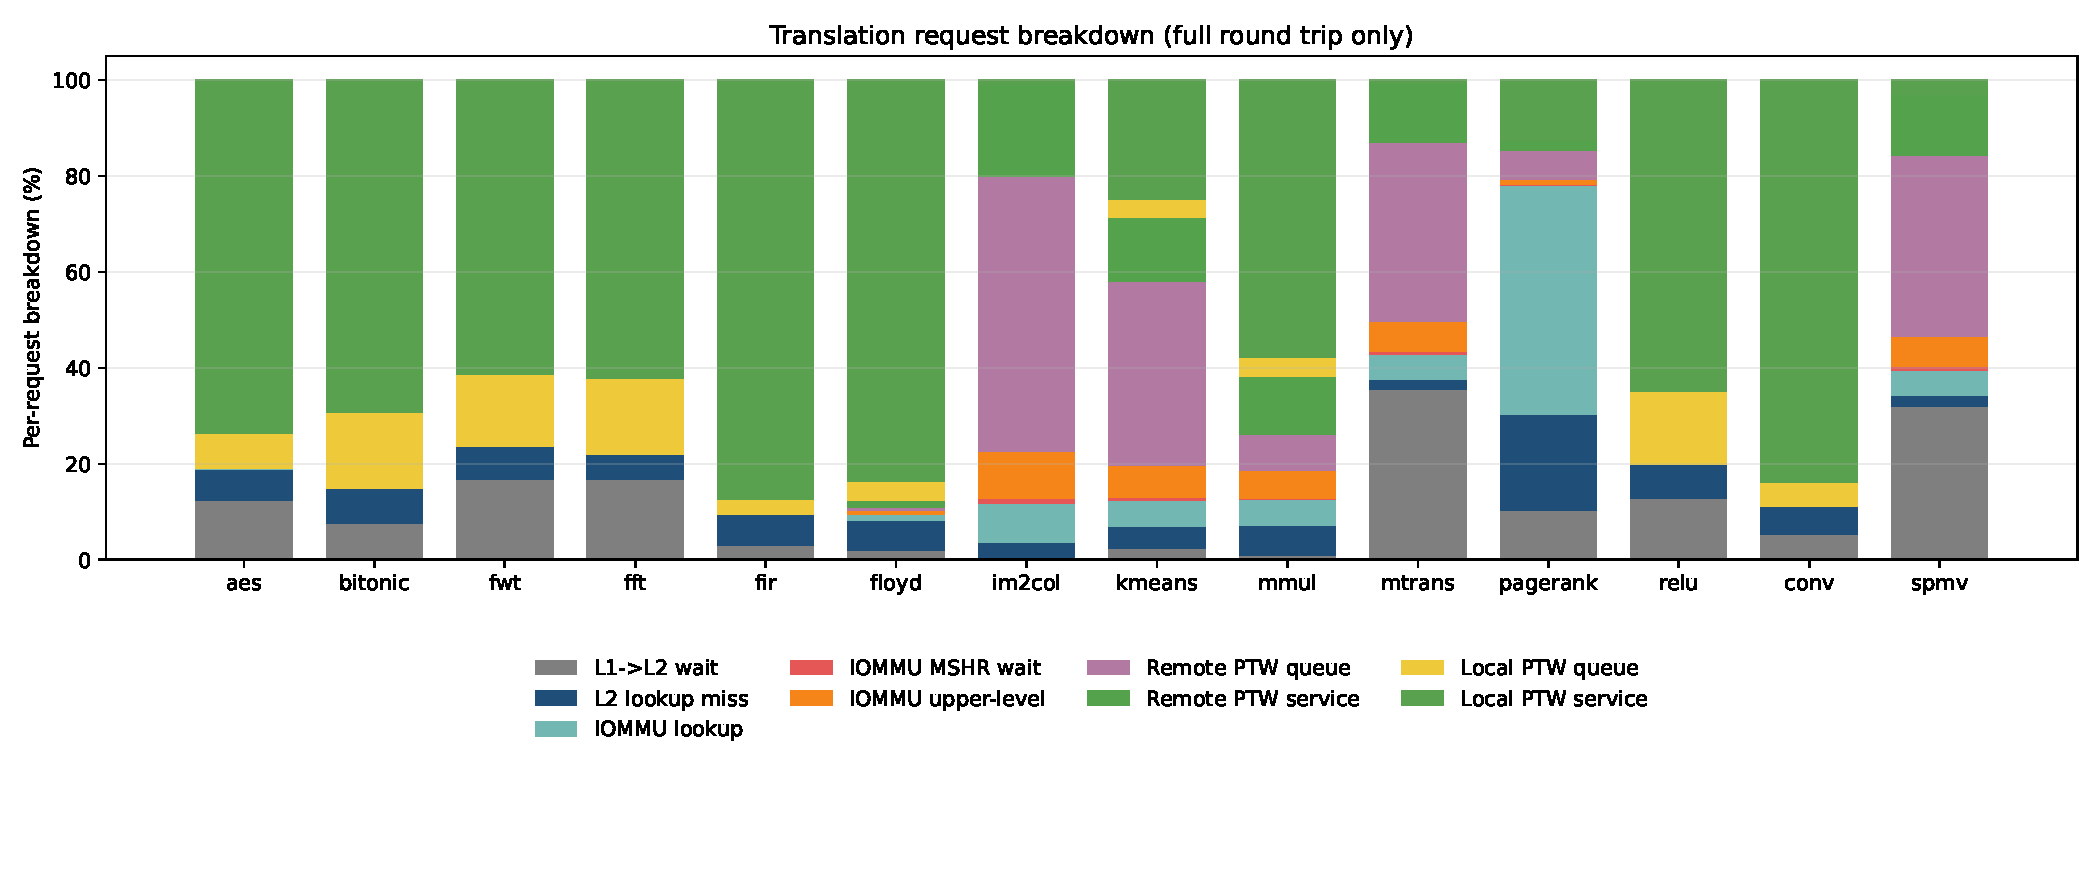
\includegraphics[width=\linewidth,height=0.48\textheight,keepaspectratio]{figures/translation_breakdown_per_request_percent_full_round_trip.pdf}
  \caption{Per-request translation breakdown after removing L2 TLB hit-only
  requests. The figure focuses on full round-trip translations and is intended
  to clarify where non-hit translation latency is spent.}
  \label{fig:full-round-trip-breakdown}
\end{figure}


\begin{thebibliography}{9}

\bibitem{shin2018neighborhood}
S.~Shin, M.~LeBeane, Y.~Solihin, and A.~Basu,
``Neighborhood-Aware Address Translation for Irregular GPU Applications,''
in \emph{Proceedings of the 51st Annual IEEE/ACM International Symposium on
Microarchitecture (MICRO)}, 2018, pp. 352--363.

\bibitem{ha2025latpc}
Y.~Ha, J.~Park, H.~Cha, J.~Lee, J.~Kim, W.~W. Ro, and Y.~Kim,
``LATPC: Accelerating GPU Address Translation Using Locality-Aware TLB
Prefetching and MSHR Compression,''
in \emph{Proceedings of the 58th IEEE/ACM International Symposium on
Microarchitecture (MICRO)}, 2025, pp. 418--431.

\end{thebibliography}

\end{document}
